\section{Gestione Utenti e Accessi}

Per la gestione delle identità e degli account degli utenti del sistema, è stato scelto \texttt{AWS Cognito}. In particolare, è stata adottata la soluzione \texttt{Cognito User Pools}, che offre un servizio completo per la gestione degli utenti, dell'autenticazione e dell'autorizzazione.

All'interno della user pool sono stati creati dei gruppi, ciascuno associato a uno dei ruoli descritti nella sezione \ref{ruoli}. 
I gruppi creati sono utilizzati per implementare un sistema di \texttt{Role-Based Access Control (RBAC)}, che consente di assegnare ai vari utenti di assumere uno o più di questi gruppi in base ai privilegi e ai permessi necessari per le loro attività.

includere definizione user:id come attributo, discusso dopo a cosa serve

\subsection{Creazione Utenti}

Una volta effettuato l'accesso utilizzando il metodo di login descritto nella prossima sezione, viene automaticamente creato un utente nella User Pool con le informazioni recuperate dall'identity provider.
Per automatizzare la creazione degli utenti nel database, l'aggiunta dei gruppi di default e l'inizializzazione dell'utente nella User Pool di Cognito, è stato individuato un trigger che può essere aggiunto alla user pool stessa. Questo Lambda trigger, noto come \href{https://docs.aws.amazon.com/cognito/latest/developerguide/user-pool-lambda-post-confirmation.html}{\texttt{post-confirmation}}, viene attivato solo al primo login riuscito di ciascun utente. Questa funzione consente di eseguire azioni personalizzate avendo a disposizione come informazioni le generalità dell'utente attraverso l'evento passato da Cognito. Di seguito è riportato il codice della funzione Lambda:

\lstinputlisting[
    language=TypeScript,
    caption={User Pool Post Confirmation Lambda Trigger},
    label={lst:postConfirmation}
]{code/cognito/postConfirmation.ts}

Inizialmente, vengono definiti un array di costanti \texttt{defaultGroups}, che contiene i gruppi di default per gli utenti, e un oggetto \texttt{userToGroupsMap}, indicizzato con le email degli utenti, che consente di associare ad alcuni utenti specifici i gruppi che devono possedere,  (righe 1-2).

La funzione richiede i seguenti servizi nel suo costruttore: \texttt{usersDao} (sez. \ref{dao}) e \texttt{CognitoGroupService}. Quest'ultimo utilizza la AWS SDK per effettuare chiamate all'API di Cognito, ma non entreremo nei dettagli di implementazione.

Essensialmente vengono compiuti i seguenti passi:

\begin{itemize}
    \item \textbf{Estrazione dei dati dell'utente dall'evento:}
    I dati dell'utente vengono estratti dall'evento attraverso la variabile \texttt{event.userName} e \texttt{event.request.userAttributes} (righe 10-12). 

    \item \textbf{Inizializzazione dei dati dell'utente:}
    Inizialmente, i dati dell'utente vengono estratti dall'evento e popolati con i valori corrispondenti (righe 13-20), che vengono quindi memorizzati nella variabile userData. Successivamente, vengono definiti i gruppi dell'utente, recuperandoli dall'oggetto \texttt{userToGroupsMap} se presenti, altrimenti utilizzando i \texttt{defaultGroups} (righe 21-22). Infine, userData viene aggiornato con i gruppi relativi (righe 24-27).
    
    \item \textbf{Assegnazione dell'utente ai gruppi:}
    Utilizzando il servizio \texttt{cognitoGroupsService}, l'utente viene aggiunto ai gruppi definiti in \texttt{userGroups} nella user pool di Cognito (righe 28-29).

    \item \textbf{Creazione dell'utente nel database:}
    Utilizzando il DAO degli utenti, l'utente viene creato nel database con le informazioni ottenute (righe 30-31).

     \item \textbf{Aggiornamento attributi utente nella UserPool:}
    Infine, utilizzando l'ID dell'utente appena creato, procedo con l'aggiornamento dell'attributo personalizzato "custom:user\_id" dell'utente nella user pool, utilizzando il servizio \texttt{CognitoGroupsService} (riga 39).
    
\end{itemize}

\subsection{Autenticazione}

\label{autenticazione}
 - specificare login dalla web app qualche parte
Il sistema Skill Manager è progettato per i dipendenti aziendali di TAI, che utilizzano Gmail come posta elettronica aziendale. Per semplificare il processo di login e sfruttare le credenziali già in loro possesso, è stata scelta la federazione con Google come Identity Provider (IdP) per la user pool di Cognito.

-- qui manca configurazione resource server, scopes, domain names, callback urls

\subsubsection{OauthFlow}
Il processo di login si basa sul framework Oauth 2.0, adottato da Cognito.

Durante la fase di creazione dei token, i gruppi a cui un utente appartiene vengono automaticamente inclusi nell'access token da Cognito sotto il claim \texttt{cognito:groups}, mentre gli attributi dell'utente nella user pool non vengono automaticamente aggiunti ai token. Pertanto, per inserire l'ID dell'utente nell'access token, è stato aggiunto un ulteriore Lambda trigger alla user pool, chiamato \href{https://docs.aws.amazon.com/cognito/latest/developerguide/user-pool-lambda-pre-token-generation.html#user-pool-lambda-pre-token-generation-accesstoken}{pre-token-generation}. Questo trigger viene attivato prima della generazione di ciascun access token e offre la possibilità di aggiungere o sovrascrivere dei custom claims e dei gruppi. La funzione riceve da Cognito le informazioni sull'utente, inclusi i gruppi e gli attributi della User Pool. 

Di seguito è presentato il codice, in cui viene estratto l'ID dell'utente dall'evento e successivamente aggiunto ai claims personalizzati dell'access token.

\lstinputlisting[
    language=TypeScript,
    caption={User Pool Pre Token Generation Trigger},
    label={lst:preTokenGeneration}
]{code/cognito/preTokenGeneration.ts}

Ecco un diagramma di sequenza che illustra il processo di login e le varie risorse coinvolte nel processo.

\begin{figure}[ht]
    \centering
    \makebox[\textwidth][c]{%
        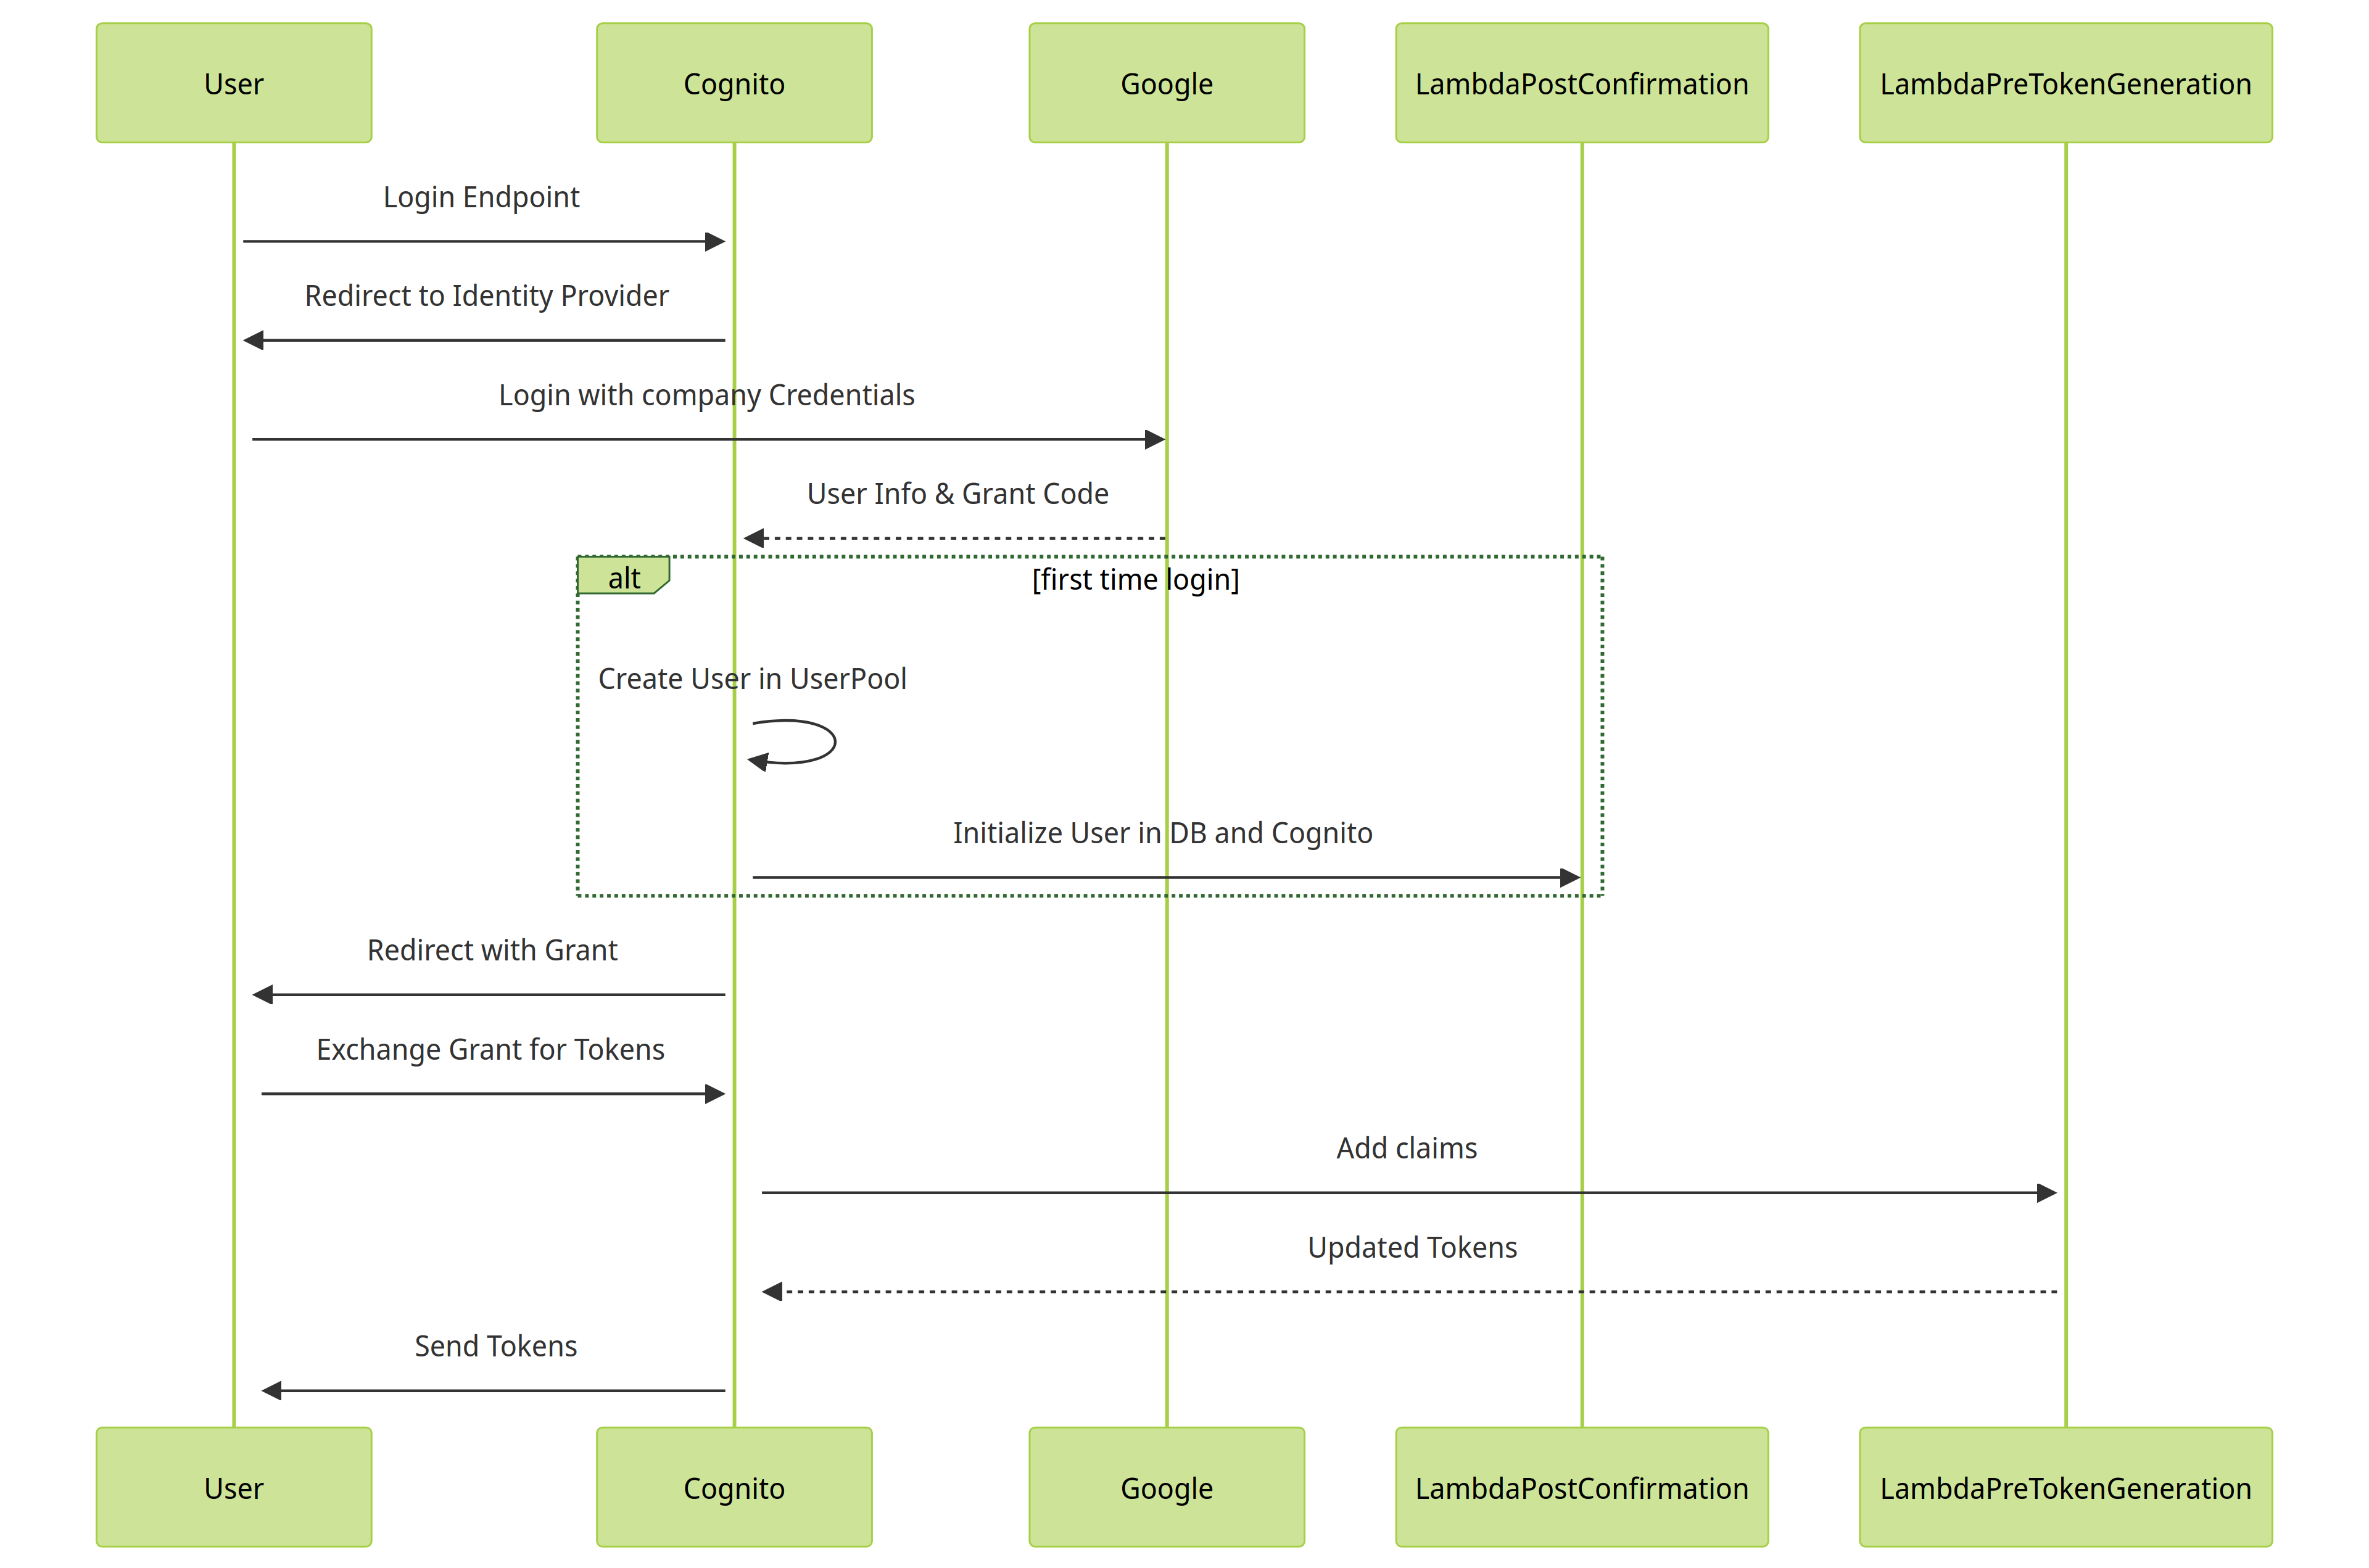
\includegraphics[width=1.1\linewidth]{immagini/oauth_flow.png}%
    }
    \caption{Diagramma di sequenza OauthFlow 2.0}
    \label{auth_sequence}
\end{figure}

\FloatBarrier


\subsection{Autorizzazione}

\label{authorizer}
Dopo aver effettuato l'accesso al sistema e ottenuto un access token (come descritto nella sezione \ref{autenticazione}), l'utente deve includerlo in tutte le richieste alla REST API per garantirne la sicurezza e l'autorizzazione.\
Per fare questo, il client aggiunge un header \texttt{Authorization} nella richiesta HTTP, con il valore \texttt{"Bearer {token}"} \cite{rfc6750}, dove {token} è l'access token ottenuto in fase di autenticazione.

\vspace{0,3cm}
Per gestire la validazione del token, è stato implementato un \texttt{Custom Authorizer} basato su una funzione Lambda. Questa funzione è stata configurata come authorizer nell'integrazione tra la lambda REST API e l'API Gateway, venendo quindi invocata prima di ogni chiamata per autorizzare la richiesta. Solo gli utenti con un token valido possono accedere al servizio. A seconda del risultato della validazione, l'authorizer genera una risposta che contiene le seguenti informazioni:

\begin{itemize}
    \item \textbf{PrincipalId:} L'ID dell'utente nella user pool, se il token è valido.
    \item \textbf{Policy document:} Un documento che specifica le azioni che l'utente è autorizzato a compiere.
    \item \textbf{Effect:} "Allow" se l'utente è autorizzato, "Deny" se non lo è.
    \item \textbf{Context:} Un oggetto opzionale che può contenere informazioni aggiuntive da trasmettere alla funzione successiva.
\end{itemize}
Queste informazioni sono utilizzate dall'API Gateway per determinare se accettare o rifiutare la richiesta del client. Questo processo costituisce il \texttt{primo strato di sicurezza} per il controllo dell'accesso alle risorse del sistema (fase 7 della imm. \ref{auth_cloud}).

Il codice dell'authorizer, che riflette i procedimenti illustrati fino ad ora, può essere consultato nell'Appendice, nella sezione \ref{lst:authorizer-codice}.

\vspace{0,3cm}

Il \texttt{secondo strato di sicurezza} è implementato dalla API, che utilizza le informazioni presenti nel context, quali gruppi e ID utente, per eseguire un'autorizzazione più granulare (fase 9 della imm. \ref{auth_cloud}, vedi dettagli nella sezione \ref{context_service}).
Queste informazioni sono contenute nell'access token, vengono recuperate dall'authorizer in fase di decodifica del token, successivo alla validazione, e poi inserite nel context.

\vspace{0,3cm}

I seguenti diagrammi illustrano l'interazione tra le varie risorse nel processo di autorizzazione di una richiesta. Nel diagramma di sequenza si assume che l'utente sia già in possesso dell'access token e sono rappresentati anche gli errori che possono essere restituiti al client. Nel secondo diagramma si presume che l'autorizzazione sia andata a buon fine.

% valutare se mettere qui la lambda pre token generation - sicuramente andrà nel diagramma dell'autorizzazione
% rivedere naming delle entità

\begin{figure}[ht]
    \centering
    \makebox[\textwidth][c]{%
        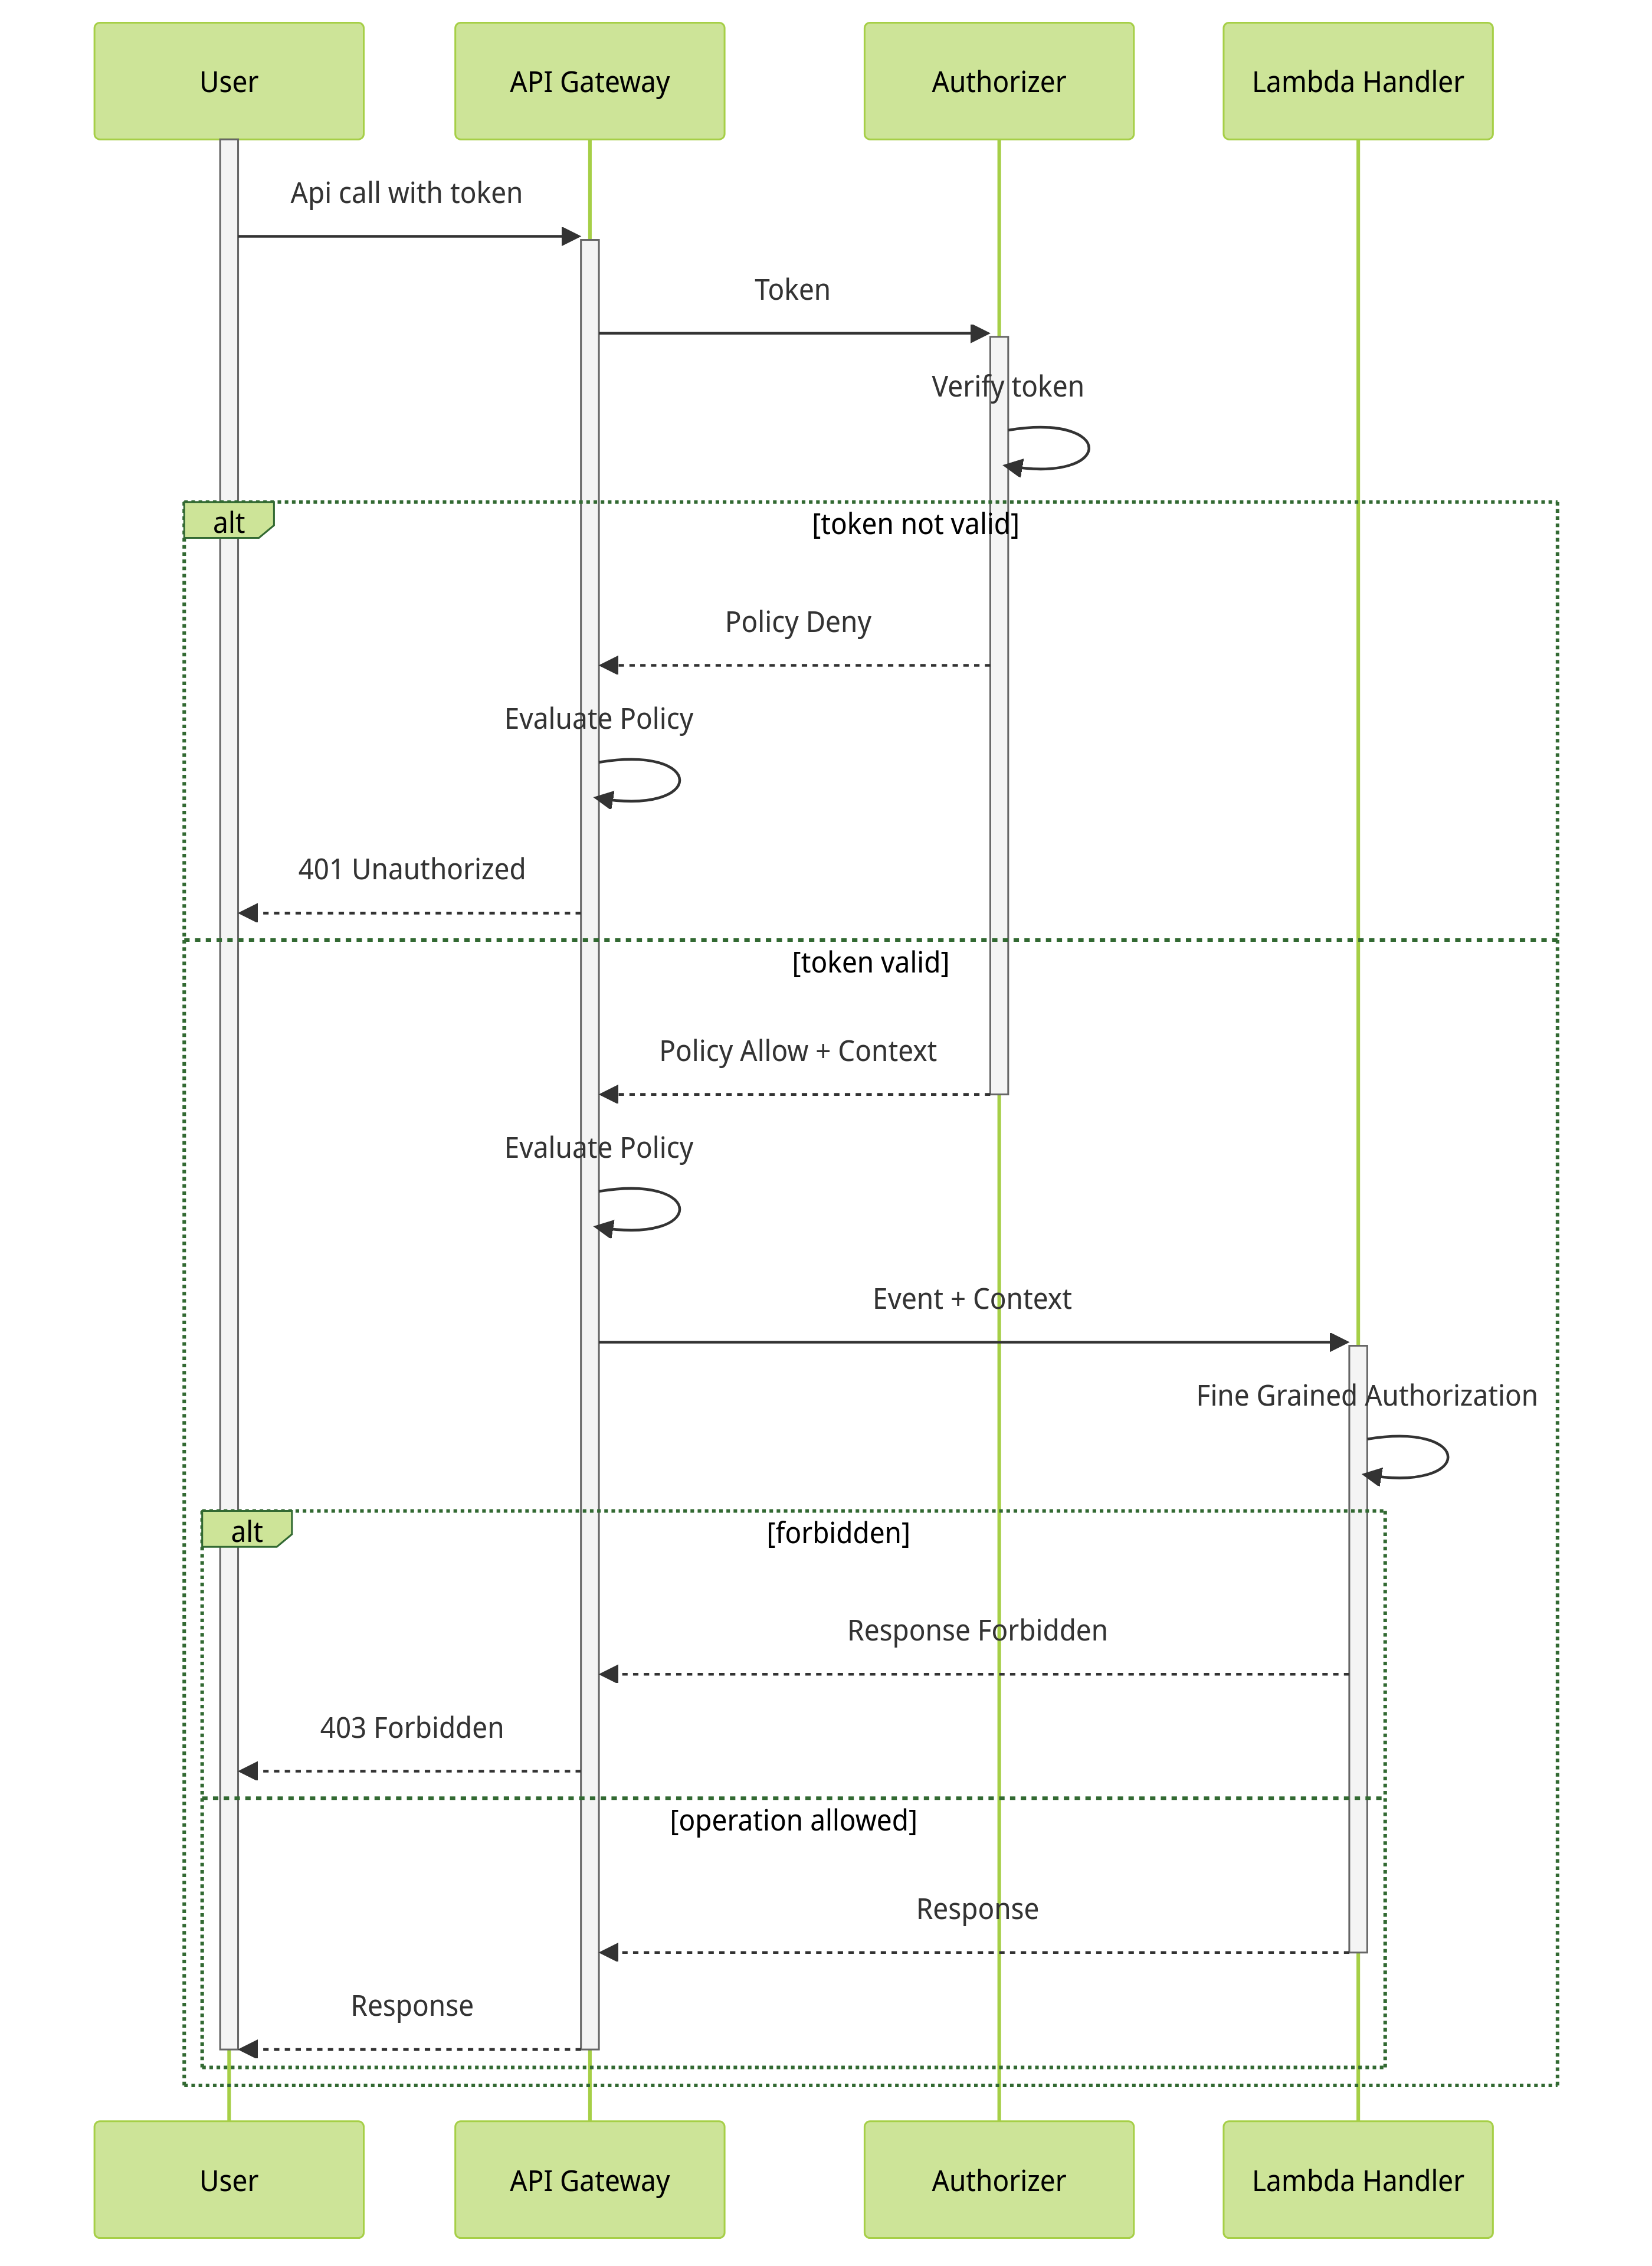
\includegraphics[width=0.9\linewidth]{immagini/Authorization_Flow.png}%
    }
    \caption{Diagramma di sequenza del flusso di autorizzazione}
    \label{auth_sequence}
\end{figure}

\FloatBarrier


\begin{figure}[ht]  
    \centering
    \makebox[\textwidth][c]{%
        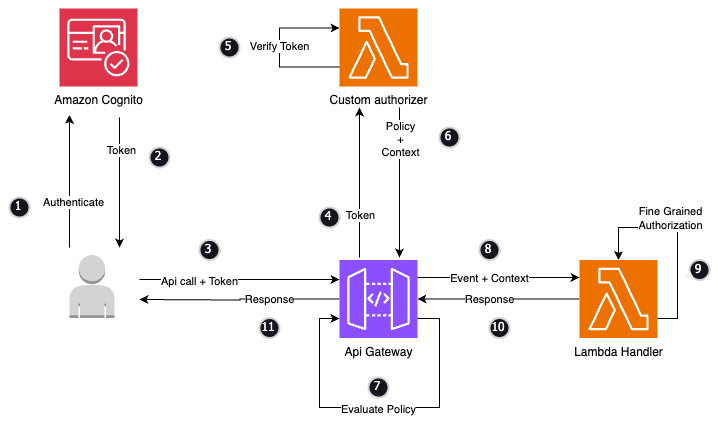
\includegraphics[width=0.9\linewidth]{immagini/AuthFlow_white.png}%
    }
    \caption{Flusso di autorizzazione del sistema andato a buon fine}
    \label{auth_cloud}
\end{figure}

\FloatBarrier

